Hamiltonian Monte Carlo is considered a state-of-the-art sampler that efficiently explores sample space by producing large jumps to successive states with low correlation, 
but suffers the need for manual tuning of the trajectory length $\epsilon L$. 
In this chapter, we will explore improvements that adaptively adjust the trajectory length. This is achieved by means of adapting both the number of Leapfrog steps $L$ using an improved sampler called the \textit{No-U-Turn} (NUTS) sampler, and an adaptive scheme for setting the step size $\epsilon$ using a \textit{dual-averaging} algorithm. We will closely follow the treatment in the original paper \cite{nuts} but adapt the notation to be consistent with the rest of this thesis.

We will start off with a discussion on how to adapt the number of Leapfrog steps using NUTS. At a high-level, NUTS starts from an initial state $(q, p)$ and simulates the Hamiltonian dynamics of the system. This is
done in the following way. Leapfrog steps are performed either forwards or backwards in time, first with a single Leapfrog step, then two Leapfrog steps, then followed by four Leapfrog steps and so on. This reiteration of the simulation is performed until the the path traced out in position space starts to double back towards itself. The states traced out can be regarded as a \textit{balanced binary tree} $\mathcal{B}$ where
each node represents a phase-space state produced by the Leapfrog integrator during the simulation. The next state of the Markov chain is sampled at random from these nodes.  

We will end the chapter with the dual averaging-scheme for adaptively setting the step size used with Leapfrog integrator. The algorithm is a modified version of a dual-averaging scheme presented by Nesterov in \cite{Nesterov2009}.


\section{The No-U-Turn Sampler}
The No-U-Turn sampler generates a set of states we may regard as a balanced binary tree which we represent with the set $\mathcal{B}$. 
We shall explain the way it is built by starting from an initial point and building up the tree gradually before we generalize the procedure. An example of a trajectory in a two-dimensional position space generated by NUTS is shown in figure \ref{fig:nuts_trajectory}. 
The initial state $(q, p)$ is defined as the the node of the tree of depth $j = 0$. We sample a direction at random in time, either forwards ($v_0 = 1$) or backwards ($v_0 = -1$) and perform a single Leapfrog step to produce a new state $(q', p')$ using the step size $\epsilon v_0$. This state represents its own little subtree of height $j = 0$ which is to be combined with the initial node to form a tree of height $j = 1$. If $v_0 = 1$, the new node is placed as the right half of the new tree. Conversely, if $v_0 = -1$, the new node is placed as the left half of the new tree. We repeat, but this time we double the number of Leapfrog steps to $L = 2$. We randomly sample the direction once more. If forwards in time ($v_1 = 1$), we initiate the Leapfrog integrator from rightmost node of the current tree (which represents the head of the trajectory in position space). If backwards in time ($v_1 = -1$), we feed the state of the leftmost node to the Leapfrog integrator (which represents the tail of the trajectory in position space) and integrate backwards in time. The new states produced with the Leapfrog integrator becomes the nodes of a subtree of height $j = 1$ which will be combined with the current tree. Again, if $v_1 = 1$, we place the new subtree as the right half of the combined tree. If $v_1 = -1$, it is placed as the left half of the combined tree. 
This procedure is carried out repeatedly. We draw a direction in time at random, and perform twice as many Leapfrog steps as the prior iteration from the rightmost node if forwards in time or from the leftmost node if backwards in time to extend the trajectory further. More precisely, given a tree of height $j$, 
\begin{enumerate}
    \item Sample a direction $v_j \sim \text{Uniform}(\{-1, 1\})$ in time. Set the step size in the Leapfrog integrator as $\epsilon \to \epsilon v_j$.
    \item Perform $2^j$ Leapfrog steps from the rightmost node if $v_j = 1$ or from the leftmost node if $v_j = -1$.  
    \item The new generated tree of height $j$ is combined with the current tree of height $j$, producing a combined tree of height $j + 1$. If $v_j = 1$, the newly generated tree becomes the right half of the combined tree. If $v_j = -1$, it becomes the left half of the combined tree.
\end{enumerate}
From a practical perspective, we cannot apply these steps repeatedly \textit{ad-infinitum} of course. At some point, we must stop the doubling of the tree and select a node which from which we obtain the position state to take the next place in the Markov chain. How this is solved is what we shall consider next.


\begin{figure}[h!]
    \centering
    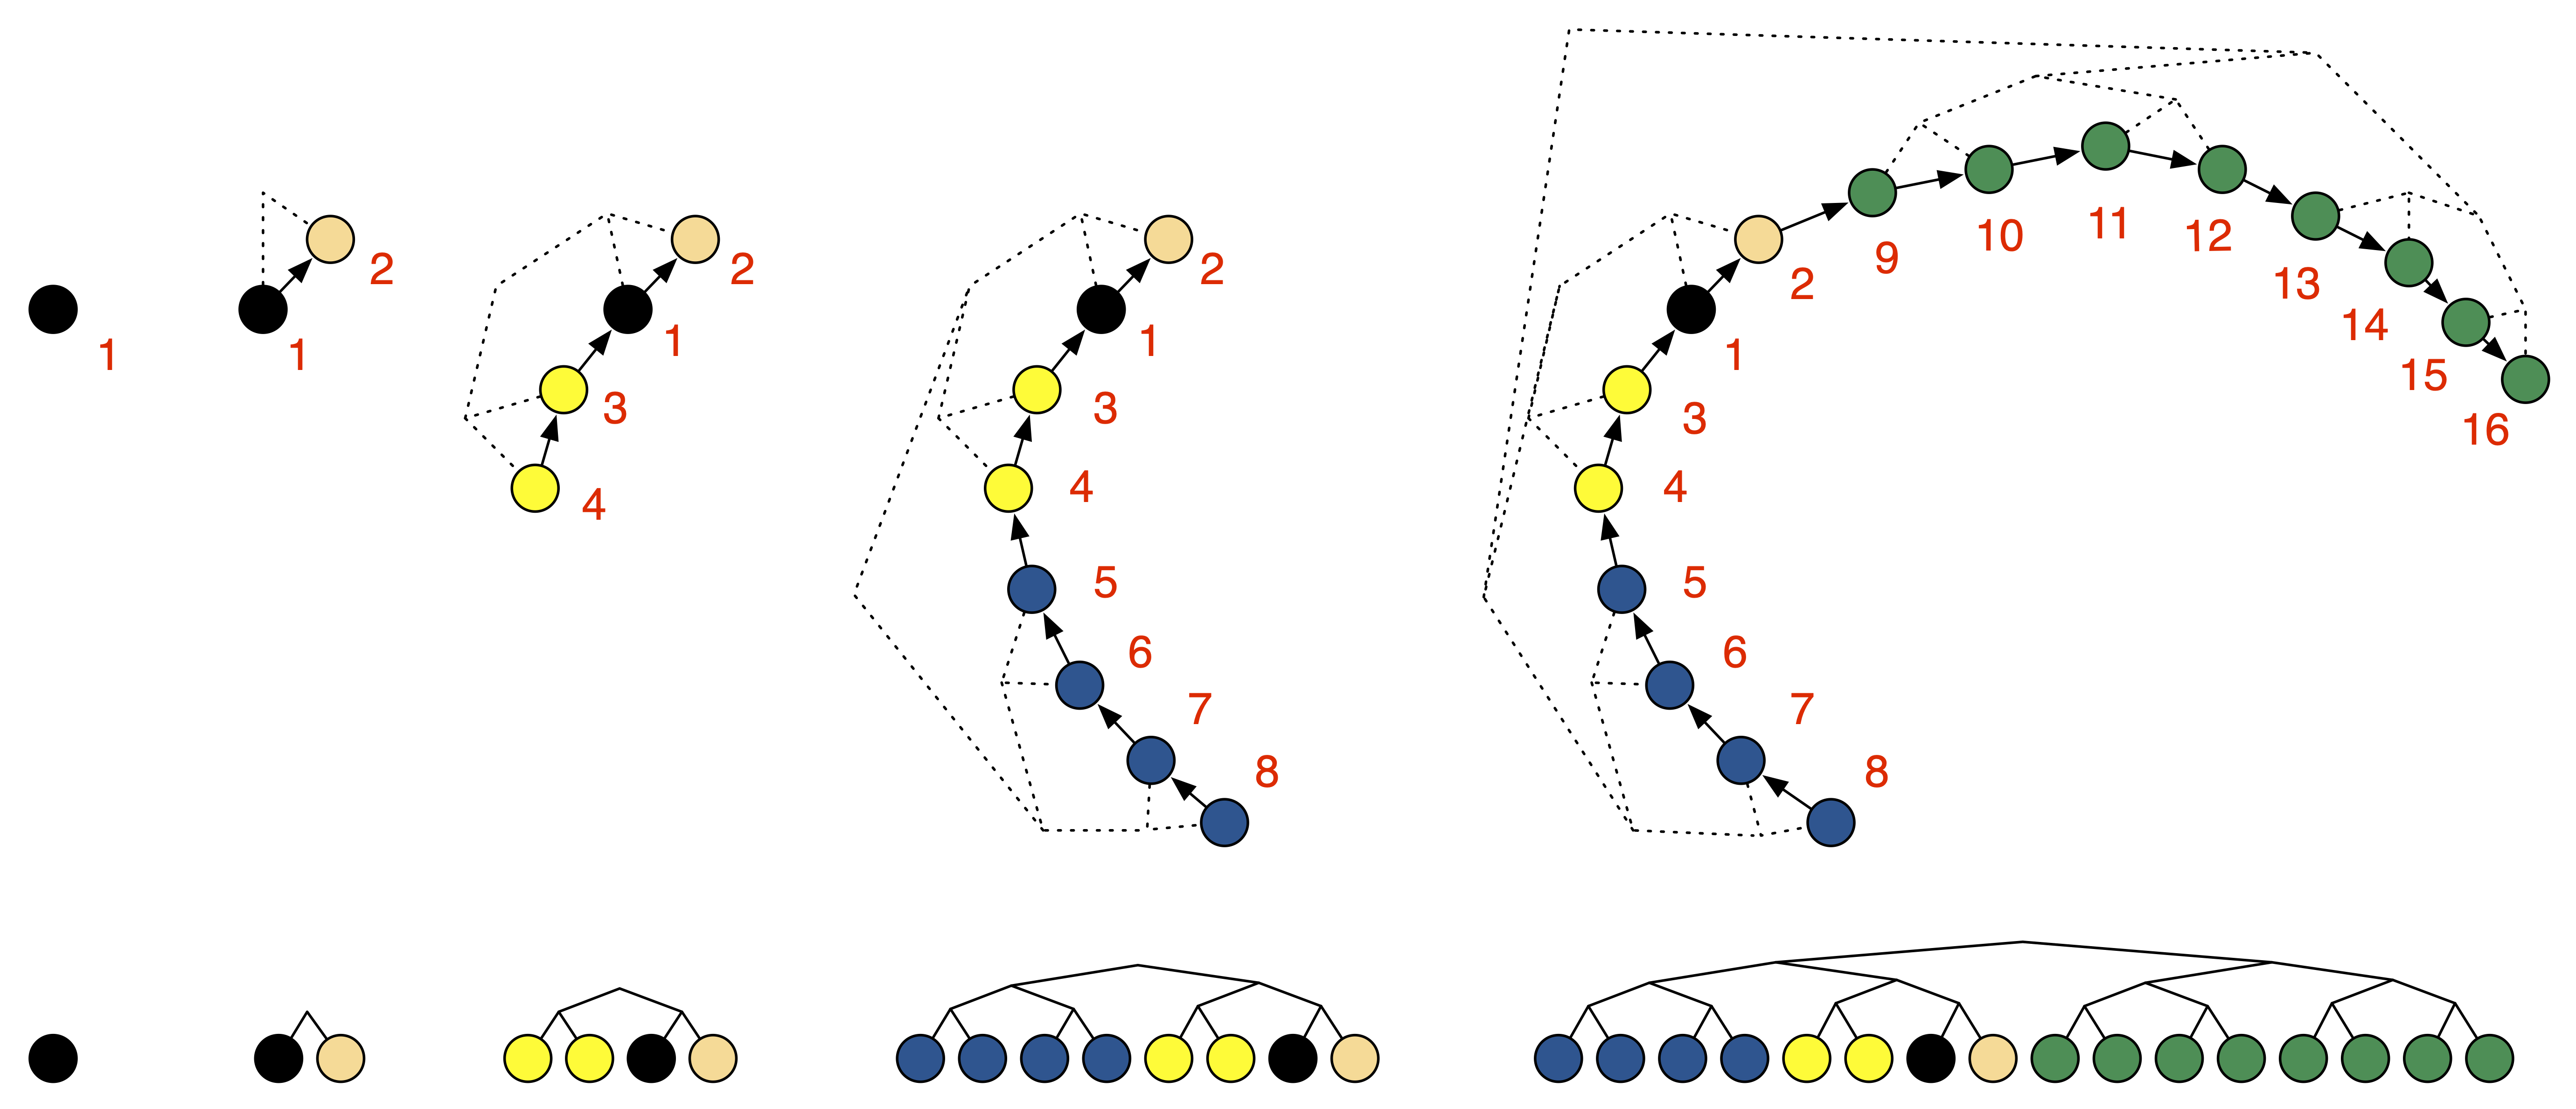
\includegraphics[scale=0.075]{figures/drawings/doubling3_with_numbering.png}
    \caption{The figure shows an example of a trajectory generated by the NUTS sampler. The top diagram displays the projection onto position space with the momenta drawn in as arrows. The bottom diagram shows the resulting balanced binary tree. The tree structure is drawn onto the trajectory as well. The numbering displays the order in which the states are generated by Leapfrog integration. The black node is the initial node. The first doubling is forwards in time and yields the rightmost node of the first binary tree. The second doubling is backwards in time and is initiated from the black node, yielding a new tree of height 2 where the left subtree is the new states (the yellow nodes). The next doubling is also backwards in time, and the Leapfrog integrator is initiated from the tail (the leftmost yellow node) performing four Leapfrog steps generating a subtree which becomes the left half of the next tree (blue nodes). The final doubling in the figure is forwards in time with $L = 8$ Leapfrog steps taken from the orange node (which was the rightmost leaf of the tree before the final doubling) which yields the green nodes. The figure is a modified version of a diagram in \cite{nuts}.}\label{fig:nuts_trajectory}
\end{figure}

\begin{comment}
    The main benefit HMC introduced over random walk Metropolis is its ability to produce large jumps in parameter space, allowing efficient exploration of the typical set. Doubling back towards other states that are already part of the trajectory is wasteful and removed the benefit HMC introduces in the first place. 
\end{comment}

\subsection{Stopping Conditions and Selection of Candidate States}
We seek a way to stop the doubling procedure that automatically does so when continuing is no longer beneficial from a computational standpoint.
Let us first consider a point we stressed in chapter \ref{chap:hmc}. If Hamilton's equations are solved exactly, the generated trajectory is confined to a hyperplane. Thus for an exact solution, the trajectory would at some point in time double back towards itself. This will likely also happen when we only approximate the solution with the Leapfrog integrator. If we continue the doubling procedure when the generated trajectory begins to double back on itself  (perform a ``U-turn''), we will revisit regions of parameter space that are already part of the binary tree, thus wasting computational resources. To avoid this, we ought to check during each doubling if such a ``U-turn'' occurs and terminate if it does. Consider an initial state $(q, p)$ and let $(q', p')$ be a point produced by the Leapfrog integrator (which is treated as a function of time). Then the change in the Euclidean distance between the positions are
\begin{equation}\label{eq:change_in_distance}
    \dv{t}\frac{\norm{q' - q}_2^2}{2} = (q' - q)^T \dv{t}  (q' - q) = (q' - q)^Tp'.
\end{equation}
If eq.~\eqref{eq:change_in_distance} evaluates to a negative number, continuing the simulation for an infinitesimal time $\dd t$ will decrease the distance between the points which is how we can detect an occurence of a ``U-turn''. The way the NUTS sampler does this, is to consider the leftmost and rightmost node of \text{any} subtree of the current tree. Let $(q^+, p^+)$ be the rightmost node and $(q^-, p^-)$ the leftmost node of any subtree. Then if 
\begin{equation}\label{eq:no_u_turn_condition}
    (q^+ - q^-)^Tp^+ < 0 \qq{or} (q^+ - q^-)^Tp^- < 0, 
\end{equation}
is fulfilled for any of the subtrees, it terminates the doubling of the tree. This is the so-called \textit{No-U-Turn condition}. We must consider two distinct cases where the stopping condition in eq.~\eqref{eq:no_u_turn_condition} is met.
\begin{enumerate}
    \item Consider a tree of height $j$. If, during the doubling to create the tree of height $j + 1$, a ``U-turn'' is detected within any of the subtrees of the new tree of height $j$, all of its states are discarded and the tree before the doubling is taken as the final tree. That is, if eq.~\eqref{eq:no_u_turn_condition} is met for any of the subtrees of the new tree, we must discard their states. The reason for this is that if we were to begin the doubling from any of these states, the No-U-Turn condition is met before we can rebuild $\mathcal{B}$ and thus we violate reversibility and inadvertently detailed balance.
    \item Consider now the combined tree after doubling. Naturally, none of the subtrees will satisfy the No-U-Turn condition because
    \begin{enumerate}
        \item The tree before doubling had not triggered the termination of the doubling procedure. Hence, none of its subtrees nor the full tree satisfy eq.~\eqref{eq:no_u_turn_condition}. 
        \item The new tree, which is the other half of the combined tree, did not trigger a termination either so none of its subtrees nor the full tree satisfy eq.~\eqref{eq:no_u_turn_condition}.
    \end{enumerate}
    The only part of the combined tree that can satisfy the No-U-Turn condition at this is point is the rightmost and leftmost nodes of the entire tree. If eq.~\eqref{eq:no_u_turn_condition} is met in this case, we terminate the doubling but no state must necessarily be discarded. After all, since the full tree is built and none of subtrees satisfy the No-U-Turn condition, we can start from any state and find a unique set of directions $\{v_j\}$ from which we can rebuild the entire tree before the No-U-Turn condition is satisfied.
\end{enumerate}

There is another case in which we want to stop the doubling procedure. If at any point, the error of the simulation becomes too large,
the states produced during the doubling process is likely to lie in a low probability region of parameter space. Continuing the simulation at this point will likely waste computational resources as states integrated from these low probability states will yield new states in a low probability region. Let $(q', p')$ be any state in the tree (including the initial state) and denote the initial state as $(q, p)$. The doubling is terminated if
\begin{equation}\label{eq:nuts_error_condition}
    H(q', p') - H(q, p) + \log \Lambda \geq \Delta_\text{max},
\end{equation}
where $\Lambda \sim \text{Uniform}(0, 1)$ is sampled in the beginning of the tree building (and is the slice variable used during Metropolis correction to accept or reject a state) and $\Delta_\text{max}$ is a tolerance which the authors of the original paper recommends to be set to $\Delta_\text{max} = 1000$ to allow the tree building to continue if the error introduced by the Leapfrog integrator is moderate. Equation~\eqref{eq:nuts_error_condition} essentially states that if the energy difference becomes too large, we terminate the tree building. The tree produced during this final doubling must be discarded and the final tree becomes the tree prior to doubling. The reasoning is the same as before; we cannot initiate the Leapfrog integrator from the states in this tree and rebuild $\mathcal{B}$ as the stopping condition in eq.~\eqref{eq:nuts_error_condition} is met before the full tree can be rebuilt.

Once the tree $\mathcal{B}$ is built, the NUTS sampler selects a \textit{candidate set} $\mathcal{C}$ from the tree where all of its elements, which we define as \textit{candidate states}, must satisfy
\begin{equation}\label{eq:nuts_acceptance}
    \frac{\pi(q', p')}{\pi(q, p)} = \exp\{-[H(q', p') - H(q, p) ]\} > \Lambda,
\end{equation}
which is the same Metropolis correction that is employed in HMC \cite{nuts_joonha_park}. The next state in the Markov chain is drawn randomly from $\mathcal{C}$. The selected state $(q', p')$ is projected onto $q'$ which is the parameter of interest that is next in line in the Markov chain. We have defined a function {\tt NUTSstep} in algorithm \ref{algo:nuts} which generates the next state $q'$ in the Markov chain given a prior state $q$, a Hamiltonian $H$ and a step size $\epsilon$.

\begin{figure}
	\begin{algorithm}[H]
	\caption{The NUTS Sampler}\label{algo:nuts}
	\begin{algorithmic}
        \Function{{\tt NUTSstep}}{$q, H, \epsilon$}
            \State Draw $p \sim \mathcal{N}(0, I)$
            \State Draw $\Lambda \sim \text{Uniform}(0, 1)$
            \State Set the initial tree $\mathcal{B} \gets \{(q, p)\}$.
            \State Set the initial candidate set $\mathcal{C} \gets \mathcal{B}$
            \For{$j \geq 1$}
                \State Draw $v_j \sim \text{Uniform}(\{-1, 1\})$
                \If{$v_j = 1$}
                    \State Do $2^j$ Leapfrog steps from the rightmost node of the current tree. Assign to $\mathcal{B}'$
                \Else
                    \State Do $2^j$ Leapfrog steps from the leftmost node of the current tree. Assign to $\mathcal{B}'$
                \EndIf
                \If{for \text{any} subtree in $\mathcal{B}'$, eq.~\eqref{eq:no_u_turn_condition} is satisfied}
                    \State Terminate building of tree and discard $\mathcal{B}'$
                \Else{
                    \State $\mathcal{B} \gets \mathcal{B} \cup \mathcal{B}'$. 
                    \If{eq.~\eqref{eq:no_u_turn_condition} is satisfied for leftmost and rightmost leaves}
                        \State Terminate building of tree.
                    \EndIf
                    \If{eq.~\eqref{eq:nuts_error_condition} is satisfied for any state in $\mathcal{B}$}
                        \State Terminate building of tree.
                    \EndIf
                }
                \EndIf
            \EndFor
            \For{$(q', p') \in \mathcal{B}$}
                \If{$\exp\{-[H(q',p') - H(q, p)]\} > \Lambda$}
                    \State $\mathcal{C} \gets \mathcal{C} \cup \{(q', p')\}$
                \EndIf
            \EndFor
            \State Draw $(q', p')$ at random from $\mathcal{C}$.
            \State \Return $q'$
        \EndFunction
	\end{algorithmic}
	\end{algorithm}
\end{figure}

\subsection{Computational Cost}
The No-U-Turn sampler introduces additional operations to keep track of whether any of the stopping conditions are met.
Equation~ \eqref{eq:no_u_turn_condition} requires $2^{j+1} - 2$ evaluations of inner products for a tree of height $j$, two inner products per subtree. 
In addition, eq.~\eqref{eq:nuts_error_condition} requires $2^j - 1$ evaluations of the Hamiltonian, and its gradient must be calculated an equal amount of times to perform Leapfrog integration similar to what is required by HMC. The additional cost of the inner products are, however, neglible for sufficiently complex models and/or large datasets as the evaluation of the Hamiltonian and its gradient will be the dominating computational cost.
Another added computational cost is the memory footprint introduced by storing the balanced binary tree. In its naive form, the memory footprint requires the order $\mathcal{O}(2^j)$ states. A more efficient solution can be found by observing that the uniform distribution over the candidate set $\mathcal{C}$ can be rewritten as 
\begin{equation}\label{eq:uniform_dist_over_C}
    p(q, p| \mathcal{B}, \mathcal{C}) = \frac{1}{\abs{\mathcal{C}}} = \frac{\abs{\mathcal{C}_\text{subtree}}}{\abs{\mathcal{C}}}\frac{1}{\abs{\mathcal{C}_\text{subtree}}},
\end{equation}
where $\abs{\cdot}$ denotes the \textit{cardinality} or the number of elements in the set and $\mathcal{C}_\text{subtree} \subseteq \mathcal{C}$ is the candidate states in a subtree of the subset of the full tree corresponding to the candidate set. Equation~\eqref{eq:uniform_dist_over_C} states that the uniform probability over $\mathcal{C}$ can be rewritten as the probability of selecting a subtree $\mathcal{C}_\text{subtree}$ from $\mathcal{C}$ times the probability of drawing a state at random from that subtree. A tree of height $j$ consists of two subtrees of height $j - 1$. From each subtree for $j > 0$, draw a state $(q, p)$ from each subtree with probability $1 / \abs{\mathcal{C}_\text{subtree}}$ to represent that tree and a give it a weight proportional to how many states of the total candidate set that belonged to that particular subtree. Starting from the initial tree of height $j > 0$, this can be performed during the doubling process for each new subtree that is generated to avoid explicit storage.  The storage requirement is thus brought down to an order of $\mathcal{O}(j)$ position-momentum states, which significantly reduces the memory footprint.

\section{Adapting the Step Size}
Now that we have established a means of adapting the number of Leapfrog steps $L$, we turn our attention to adapting the step size $\epsilon$. We will employ a dual-averaging algorithm as in \cite{nuts}, which is a version of the stochastic convex optimization algorithm presented by Nestrov in \cite{Nesterov2009}. The algorithm we use is better suited for the MCMC methods used in this thesis.

Let $f_t$ be a quantity calculated from the Markov chain at iteration $t$ for $t\geq 1$. For our purposes, this quantity will be related to the acceptance probability $a_t$ at iteration $t$ computed using eq.~\eqref{eq:hmc_acceptance} from the HMC sampler and a target acceptance probability $\delta$ through
\begin{equation}
    f_t = \delta - a_t.
\end{equation}
Let $x \in \mathbb{R}$ be a tunable parameter of the MCMC algorithm. This parameter will in our case be a function of the step size $\epsilon$, which is the parameter we want to tune. But for numerical stability, we will use $x = \ln \epsilon$. Define the expectation of $f_t$ as 
\begin{equation}
    f(x) = \lim_{T\to\infty} \frac{1}{T}\sum_{t=1}^T \mathbb{E}[f_t|x].
\end{equation} 
The objective is to adapt $x$ such that $f(x) \to 0$, which will bring the average of the acceptance probabilities $a_t$ towards its target acceptance probability $\delta$. To this end, we employ the update scheme
\begin{equation}\label{eq:update_scheme}
    \begin{split}
        x_{t+1} & \gets \mu - \frac{\sqrt{t}}{\gamma}\frac{1}{t + t_0}\sum_{i=1}^t f_t, \\
        \bar{x}_{t+1} & \gets \eta_t x_{t+1} + (1 - \eta_t)\bar{x}_t,
    \end{split}
\end{equation}
with $x_1 = \bar{x}_1$. Here $\mu$ is a free parameter which $x_t$ is shrunk towards, $\gamma > 0$ is a free parameter expressing the rate of shrinkage, $t_0$ is introduced for numerical stability of the iterates $x_t$ and $\eta_t$ is a step size schedule dependent on $t$ that satisfies
\begin{equation}
    \sum_{t=1}^\infty \eta_t = \infty \qq{and} \sum_{t=1}^\infty \eta_t^2 < \infty,
\end{equation}
which can be achieved by choosing
\begin{equation}\label{eq:step_size_schedule}
    \eta_t = t^{-k} \qq{for} k \in (1/2, 1].
\end{equation}
The update scheme in eq.~\eqref{eq:update_scheme} will converge $x_t$ towards a fixed value. We can see this by considering large $t$ and
\begin{equation}
    \begin{split}
        x_{t+1} - x_t & = -\frac{\sqrt{t+1}}{\gamma} \frac{1}{t+1+t_0}\sum_{i=1}^{t+1}f_i + \frac{\sqrt{t}}{\gamma} \frac{1}{t+t_0}\sum_{i=1}^{t}f_i \\
        & \sim -\frac{1}{\gamma}\frac{1}{\sqrt{t}}f_{t+1} \to 0 \qq{as} t \to \infty,
    \end{split}
\end{equation}
as long as $f_t$ is bounded. As long as $x_t$ is bounded (which we just established) and $f(x)$ is a nondecreasing function of $x$, it can be shown that the update scheme in eq.~\eqref{eq:update_scheme} guarantees that $f(\bar{x}_t) \to 0$ as $t \to \infty$.

The reasoning for using dual-averaging of $\bar{x}_t$ as opposed to just averaging $x_t$ directly is that the Markov chain is finite and the dual-averaged $\bar{x}_t$ with $k < 1$ in the step size schedule from eq.~\eqref{eq:step_size_schedule} gives more weight to more recent iterations in the chain. This is desirable since the ideal step size during the initial Markov chain may be widely different from the ideal step size once the Markov chain converges to the stationary distribution. For any $k \in (1/2, 1]$ it can be shown that $\bar{x}_t$ eventually converges to the average of $x_t$ for a long enough chain. Thus for a finite number of adaptation steps $M$, we obtain an optimal value of the step size through
\begin{equation}\label{eq:optimal_step_size}
    \epsilon_\text{opt} = \log^{-1}(\bar{x}_M).
\end{equation}

To adapt the step size in standard HMC, we define $f_t$ as 
\begin{equation}\label{eq:f_hmc}
    f_t = \delta - a_t^\text{HMC},
\end{equation}
where $a_t^\text{HMC}$ is as in eq.~\eqref{eq:hmc_acceptance}. Then we set $x = \log \epsilon$ and apply the updates in eq.~\eqref{eq:update_scheme} for a finite number of steps $M$. Adapting the step size in NUTS is a little more complicated as there is no single Metropolis-correction step during the generation of the next state in the Markov chain. Instead, we calculated 
\begin{equation}\label{eq:nuts_acceptance}
    a_t^\text{NUTS} = \frac{1}{\abs{\mathcal{B}_\text{final}}}\sum_{(q', p') \in \mathcal{B}_\text{final}} \exp\{-[H(q',p') - H(q, p)]\},
\end{equation}
where $(q, p)$ are the initial state of the tree doubling and $\mathcal{B}_\text{final}$ denotes the set of states produced during the final doubling of the NUTS sampler. Thus, when the dual-averaging scheme is applied to the step size used in the NUTS sampler, the average of the acceptance probability of all the states produced during the final doubling is used instead. 
Then $f_t$ for NUTS is defined as 
\begin{equation}
    f_t = \delta - a_t^\text{NUTS}.
\end{equation}

Generalizing then, and let $a_t$ be defined either by eq.~\eqref{eq:hmc_acceptance} if the sampler is HMC or eq.~\eqref{eq:nuts_acceptance} if the sampler is NUTS. Then the algorithm can be summarized as in algorithm \ref{algo:dual_step_size_adaptation}. The algorithm performs $T$ adaptation steps with a sampler $S$ which is assumed to take in a state $q$ and return a new state $q'$ and the corresponding acceptance probability $a$ for either HMC or NUTS.


\begin{figure}[H]
	\begin{algorithm}[H]
	\caption{Dual Averaging Step Size Adaptation}\label{algo:dual_step_size_adaptation}
	\begin{algorithmic}
        \State Parameters:
        \State $T$: Number of adaptation steps.
        \State $S$: Sampler of the form $S(q) \mapsto q', a$. (Either HMC or NUTS)
        \State $q$: Initial state of Markov chain.
        \State $\epsilon$: Initial step size.
        \State $\mu, \gamma, t_0, k$: Free hyperparameters of the algorithm discussed in the text. 
        \Function{{\tt DualAveragingStepSizeAdaptation}}{$T, S, q, \epsilon, \mu, \gamma, t_0, k$}
            \State Set the initial values:
            \State $x_1 \gets \log \epsilon$
            \State $\bar{x}_1 \gets x_1$
            \State $q_t \gets q$
            \State Perform $T$ iterations adapting $x$ with $\delta$ as target acceptance probability:
            \For{$t=1, \ldots, T$}
                \State $q_{t+1}, a_t \gets S(q_t)$ \Comment{Draw next sample and get acceptance probability}
                \State $f_t \gets \delta - a_t$ 
                \State $\eta_t \gets t^{-k}$ \Comment{Step size schedule}
                \State $x_{t+1} \gets \mu - \frac{\sqrt{t}}{\gamma(t + t_0)}\sum_{i=1}^t f_i$ \Comment{First step of update scheme in eq.~\eqref{eq:update_scheme}}
                \State $\bar{x}_{t+1} \gets \eta_t x_{t+1} + (1 - \eta_t)\bar{x}_t$ \Comment{Second step of update scheme in eq.~\eqref{eq:update_scheme}}
            \EndFor
            \State $\epsilon_\text{opt} \gets \log^{-1}(\bar{x}_T)$ \Comment{Apply inverse of log to get optimal step size}
            \State \Return $q_T, \epsilon_\text{opt}$ \Comment{Return the final state and the optimal step size}
        \EndFunction
	\end{algorithmic}
	\end{algorithm}
\end{figure}
